\documentclass[t]{beamer}
\usetheme{hkl}

\title{distributions}
	\author{François Briatte \& Ivaylo Petev}
	\date{Week~\#4}

\begin{document}

  \frame[plain]{
		\titlepage\\[7.25em]
		\begin{columns}[T]
			\column{.4\textwidth}
				\tableofcontents[hideallsubsections]
			\column{.5\textwidth}
				\href{http://www.vanityfair.com/society/features/2011/05/top-one-percent-201105}{
\includegraphics[width=\textwidth]{ows-99-percent}}
		\end{columns}
	}
	%
	%

	%
	%
	\section{Histograms}
	%
	%
	
	\begin{frame}[t]{\red{Frequencies} of a categorical variable}

		\begin{center}
			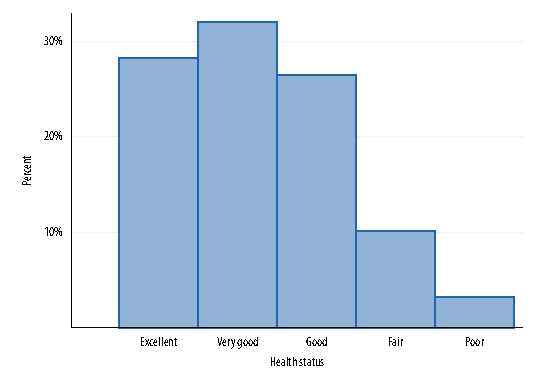
\includegraphics[height=.8\textheight]{histogram-1-discrete}
		\end{center}

	\end{frame}
	%
	%

	\begin{frame}[t]{\red{Fractions} of a continuous variable}

		\begin{center}
			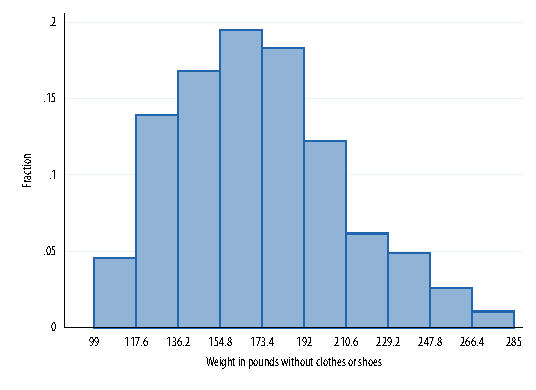
\includegraphics[height=.8\textheight]{histogram-2-fraction}
		\end{center}

	\end{frame}
	%
	%

	\begin{frame}[t]{\red{Distribution} of a variable}

		\begin{center}
			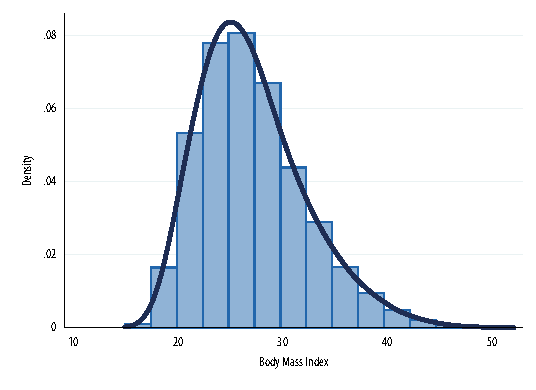
\includegraphics[height=.8\textheight]{histogram-3-density}
		\end{center}

	\end{frame}
	%
	%

	\begin{frame}[t]{Histograms}
		
	  \begin{block}{Plot the distributions of \red{continuous variables}}
			
			\begin{itemize}
				\item Use \textbf{histograms} for distributions %
					\hfill \code{hist}
				\item Use \textbf{options} for better results %
					\hfill \code{hist, bin(10) norm}
				\item Use \textbf{box plots} when there are outliers %
					\hfill \code{gr (h)box}
			\end{itemize}
	  \end{block}
	
	  \begin{block}{Split distributions with \red{categorical variables}}
						
			\begin{itemize}
				\item Plot \textbf{by} categories %
					\hfill \code{hist, by(...)}
				\item Plot \textbf{over} categories %
					\hfill \code{gr (h)box, over(...)}
				\item Plot \textbf{bars} to compare means %
					\hfill \code{gr (h)bar, over(...)}
			\end{itemize}
	  \end{block}
		
	\end{frame}
	%
	%
	
	%
	%
	\section{Descriptors}
	%
	%

	%
	%
	\subsection{Central tendency: mean, median, mode}
	%
	%

	\begin{frame}[t]{Descriptors}

	  \begin{block}{Measures of central tendency}
  	
			\begin{itemize}
				\item \textbf{Mean:} the `average' value
				\item \textbf{Median:} the `middle' value
				\item \textbf{Mode:} the `most frequent' value
			\end{itemize}
	
	  \end{block}
  
	  \begin{block}{Usage}
			\begin{itemize}
				\item Use the \textbf{mean} for continuous variables %
					\hfill \code{su}
				\item Use the \textbf{median} when there are outliers %
					\hfill \code{su, d}
				\item Use the \textbf{mode} for categorical variables %
					\hfill \code{fre}
			\end{itemize}
	  \end{block}

	\end{frame}
	%
	%
		
	\begin{frame}[t]{Mean and median}

	  \begin{block}{Arithmetic mean}
  	
			$$\red{\bar{X}} = \frac{X_1 + X_2 + \cdots + X_N}{N} = %
				\red{\frac{1}{N} \sum_{i = 1}^N X_i}$$
	
	  \end{block}
  
	  \begin{block}{Median value}
			\begin{itemize}
				\item \textbf{Quartiles:} four segments each containing %
				25\% of the data
				\item \textbf{Percentiles:} 100 segments each containing %
				1\% of the data
				\item \textbf{Median:} \red{50th percentile} (upper bound of `Q2') 
			\end{itemize}
	  \end{block}

	\end{frame}
	%
	%

	%
	%
	\subsection{Skewness a.k.a. symmetry}
	%
	%

	\begin{frame}[t]{Skewness a.k.a. symmetry}

		\begin{columns}[c]
			\column{.65\textwidth}
			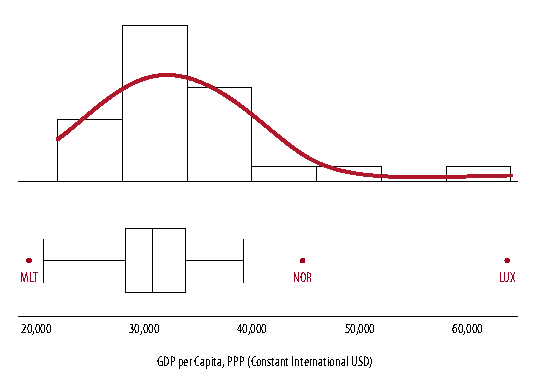
\includegraphics[width=\textwidth]{histogram-boxplot-gdpc}
			
			\column{.25\textwidth}
			\href{http://vita.had.co.nz/papers/boxplots.html}%
				{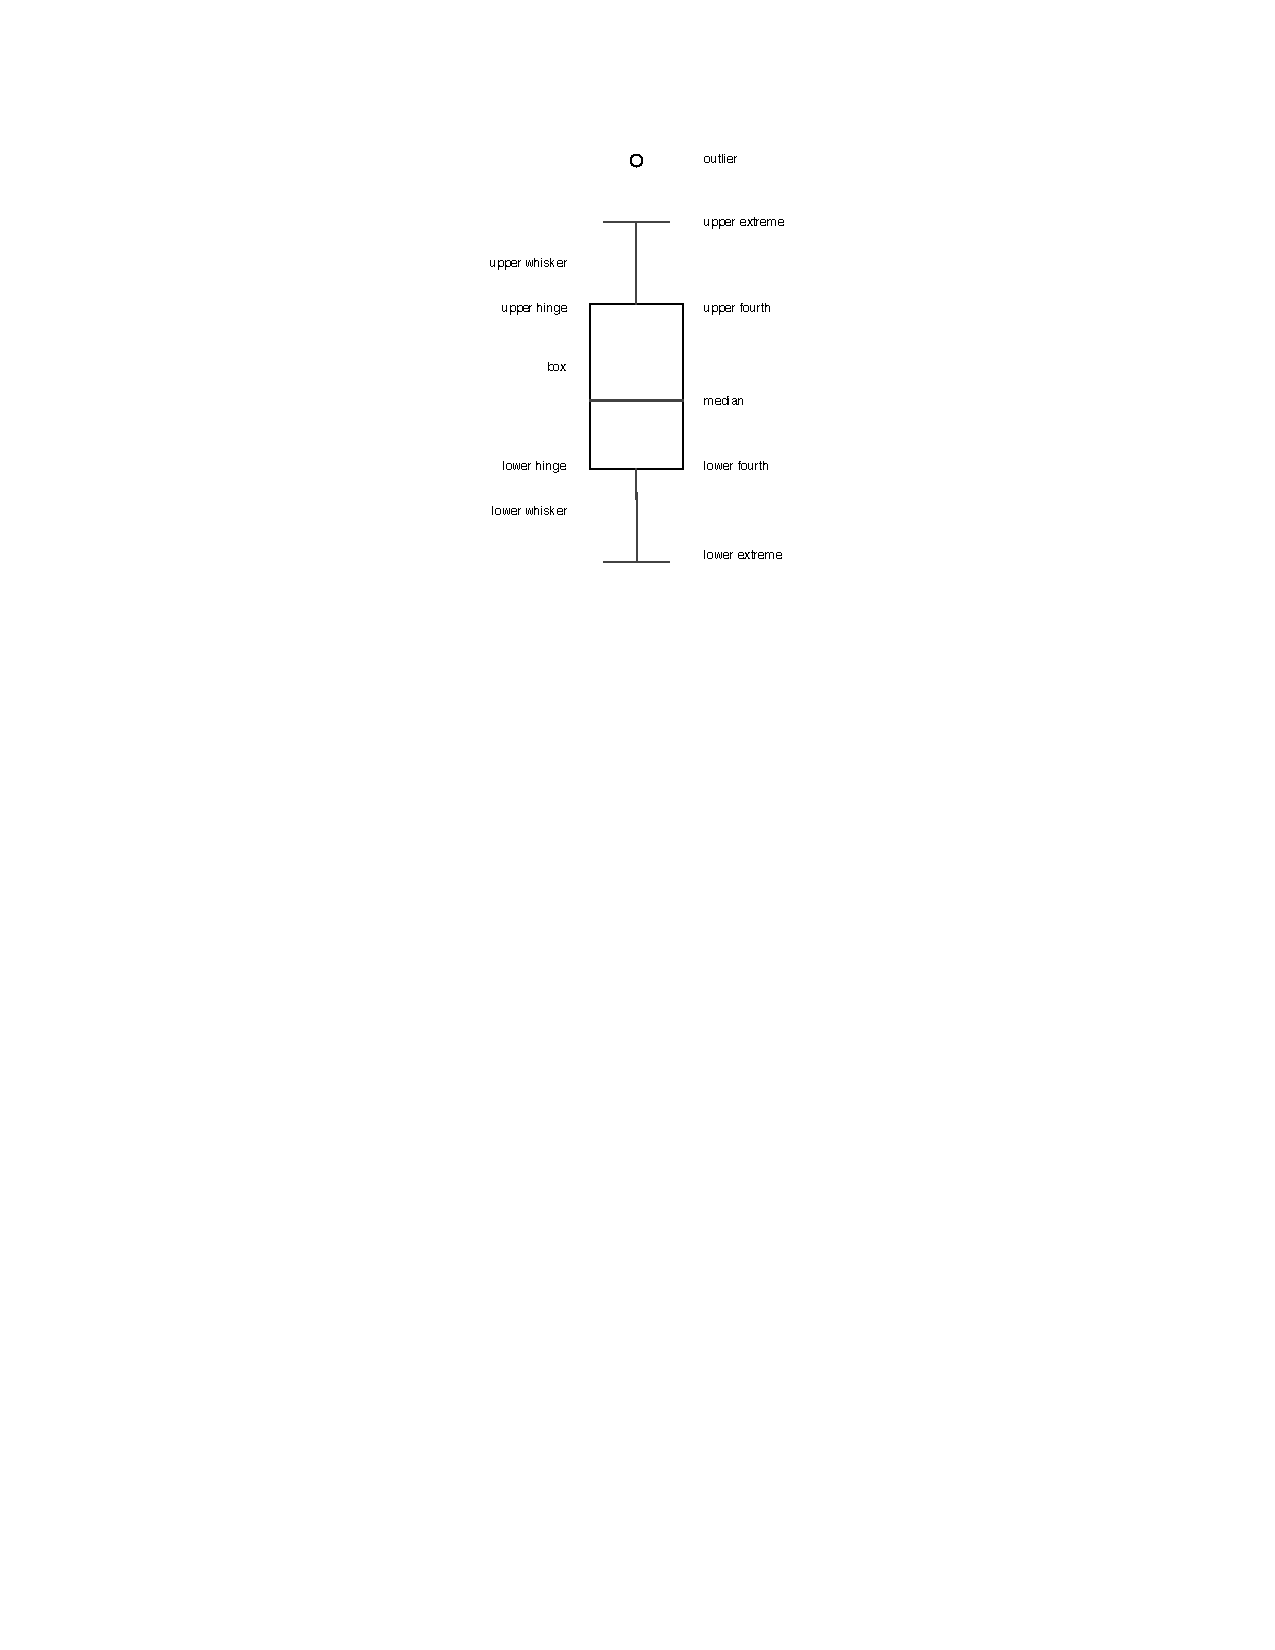
\includegraphics[width=\textwidth]{boxplot-construction}}
		\end{columns}
		
		\vspace{1em}
		
		\begin{itemize}
			\item \textbf{Positive skew:} %
				`right tail' of higher values, $\textsf{mean} > \textsf{median}$
			\item \textbf{Negative skew:} %
				`left tail' of lower values, $\textsf{mean} < \textsf{median}$
		\end{itemize}
		
	\end{frame}
	%
	%
	
	%
	%
	\subsection{Variability}
	%
	%
	
  
  \begin{frame}[c]{Variability}

		\begin{center}
			\href{http://www.phdcomics.com/comics.php?f=1563}{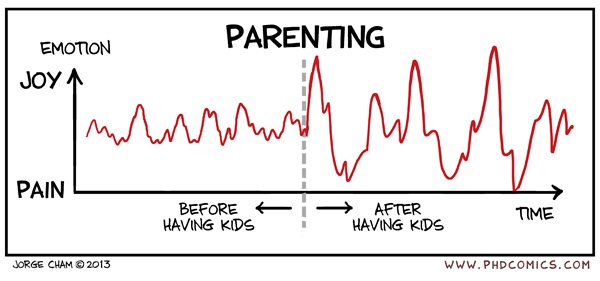
\includegraphics[width=.8\textwidth]{phdcomics-parenting}}
    \end{center}
		  
  \end{frame}
  %
  %
	
	\begin{frame}[t]{Variability}

		\begin{block}{Measures of dispersion}
			\begin{itemize}
				\item $X_{max} - X_{min}$: \textbf{range} (in `natural' units of $X$)
				\item $Var_X$: \textbf{squared distances from the mean} (summed over $N$)
				\item $SD_X$: \textbf{dispersion} (compound square root of variance by $N$)
			\end{itemize}
		\end{block}
	
	  \begin{block}{Variance and standard deviation}

			$$Var_X = \sigma^2 = \red{\frac{1}{N}} \sum_{i=1}^N (\red{X_i - \bar X})^2 \quad SD_X = \sigma = \sqrt{\red{\frac{1}{N}} \sum_{i=1}^N (X_i - \bar X)^2}$$

		\end{block}
	
	\end{frame}
	%
	%
	
	%
	%
	\section{Normal distribution}
	%
	%
	
	%
	%
	\subsection{Properties}
	%
	%
	
	\begin{frame}[t]{Normal distribution $\mathcal{N}(\mu,\,\sigma^2)$}
	
	\begin{block}{Properties}
		
		\begin{itemize}	
			\item $\mathcal{N}(\mu, \sigma^2):$ \red{symmetric} and \red{unimodal}
			\item $\mathcal{N}(\mu, \sigma^2):$ \red{mean $=$ median $=$ mode}
			\item $\mathcal{N}(0, 1):$ \red{standard normal distribution}
		\end{itemize}

	\end{block}

	\begin{center}
		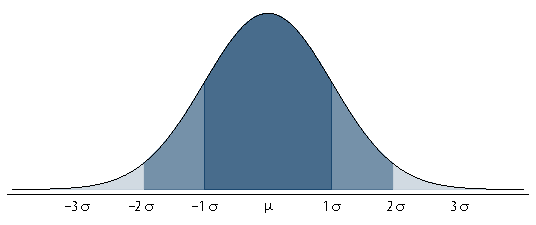
\includegraphics[width=.8\textwidth]{normal-distribution.pdf}
	\end{center}
	
	\end{frame}
	%
	%
	
	%
	%
	\subsection{Assessment}
	%
	%
	
	\begin{frame}[t]{Normality assessment}
		
	\begin{block}{Visual assessment}
	
		\begin{itemize}
			\item Distributions \hfill %
				\code{hist, normal}, \code{kdensity}, \code{gr (h)box}
			\item Diagnostics \hfill %
				\code{symplot}, \code{qnorm}, \code{(g)ladder}
		\end{itemize}

	\end{block}

	\begin{block}{Formal assessment}
	
		\begin{itemize}
			\item Use \code{su x, d} to assess the symmetry %
			  (\red{$skewness \sim 0$}) %
				and `peakedness' (\red{$kurtosis \sim 3$}) of a variable.
			\item Use \code{tabstat x y, s(skew kurt) c(s)} %
				to compare a variable with its transformation (often to log-units).
		\end{itemize}

	\end{block}
		
	\end{frame}
	%
	%

	\begin{frame}[t,plain]
		
		\vspace{.3\paperwidth}
		\begin{center}
			{\Large Next time, \red{The Prophecy.}}\\
		\end{center}
		
		\vspace{1em}
		\begin{flushright}
			
\includegraphics[scale=.3]{longcat-white.jpg}		
		\end{flushright}

	\end{frame}
	%
	%
	
	%
	%
	\section{Practice}
	%	
	%

	%
	%
	\subsection{Example: NHIS dataset}
	%
	%
	
	\begin{frame}[t]{Practice: \red{NHIS dataset}}

		$$\mathsf{Body~Mass~Index} = \frac{\mbox{mass} \ \mbox{(kg)}}{\left( \mbox{height}(\mathsf{m})\right)^2} = \frac{\mbox{mass} \ \mathsf{(lb)} \times 703}{\left(\mbox{height} (\mathsf{in})\right)^2}$$
		
		\vspace{1em}

		\begin{itemize}
			\item For \textbf{normal weight} adults, $18.5 < \mathsf{BMI} < 25$.
			\item For \textbf{overweight} adults, $25 \leq \mathsf{BMI} < 30$.
			\item For \textbf{obese }adults, $\mathsf{BMI} \geq 30$.		
		\end{itemize}

		\vspace{1em}
		
    Data:
	
			\begin{columns}[c]
				\column{.725\textwidth}
				
				\begin{itemize}
					\item National Health Interview Survey (NHIS)
					\item Sample: U.S. adult population, 2009
				\end{itemize}
	
				\column{.2\textwidth}
				
\includegraphics[width=\textwidth]{logo-nhis}
			\end{columns}
	
	\end{frame}
	%
	%
	
	%
	%
	\subsection{Practice session}
  %
  %
  
	\begin{frame}[t]{Practice session}

    \begin{block}{Class}
      \comm{Get the do-file for this week.}\\
      \code{srqm fetch week4.do}\\
      
			\comm{Open to read and replicate.}\\
			\code{doedit code/week4}\\    
    \end{block}

    \begin{alertblock}{Coursework}
      \begin{itemize}
	       \item Finish the do-file and read all comments at home.
	       \item Follow instructions on top of the code.
	       \item Prepare questions in your group's draft do-file.
      \end{itemize}
    \end{alertblock}
    		
	\end{frame}
  %
  %
	
  %
  %
  \subsection{Exercise}
  %
  %
  
  \begin{frame}{Exercise}

    \begin{exampleblock}{Ex~4.1. Quality of Government 2011}
      \begin{enumerate}
        \item What countries have \emph{much} more females in government?
        \item How is the female-to-male income ratio distributed?
        \item Same question with confidence variables (\code{d wvs\_e069*}).
				\item Plot the Gini coefficient over quartiles of GDP per capita.
      \end{enumerate}
    \end{exampleblock}
		
    \begin{block}{Tips}
      \begin{itemize}
        \item Label outliers: \code{gr hbox x, mark(1, mlab(ccodealp))}
        \item Get quartiles: \code{xtile qx = x, nq(4)}
      \end{itemize}
    \end{block}

  \end{frame}
  %
  %  
	
\end{document}